\documentclass[a4paper,10pt]{article}
\usepackage[utf8]{inputenc}
\usepackage[T1]{fontenc}
\usepackage{uarial}
\renewcommand{\familydefault}{\sfdefault}
\usepackage[top=0.25in, bottom=0.25in, left=0.35in, right=0.35in]{geometry}
\usepackage[colorlinks=true, linkcolor=blue, urlcolor=blue]{hyperref}
\usepackage{graphicx}
\usepackage{tikz}
\usepackage{xcolor}
\usepackage{enumitem}

% Reduce spacing of all itemize bullet lists to match reference design
\setlist[itemize]{itemsep=0pt, parsep=0pt, topsep=1pt, partopsep=0pt, leftmargin=1.2em}

\pagestyle{empty}

\begin{document}
\noindent
\begin{minipage}[c]{0.13\textwidth}
  \begin{center}
   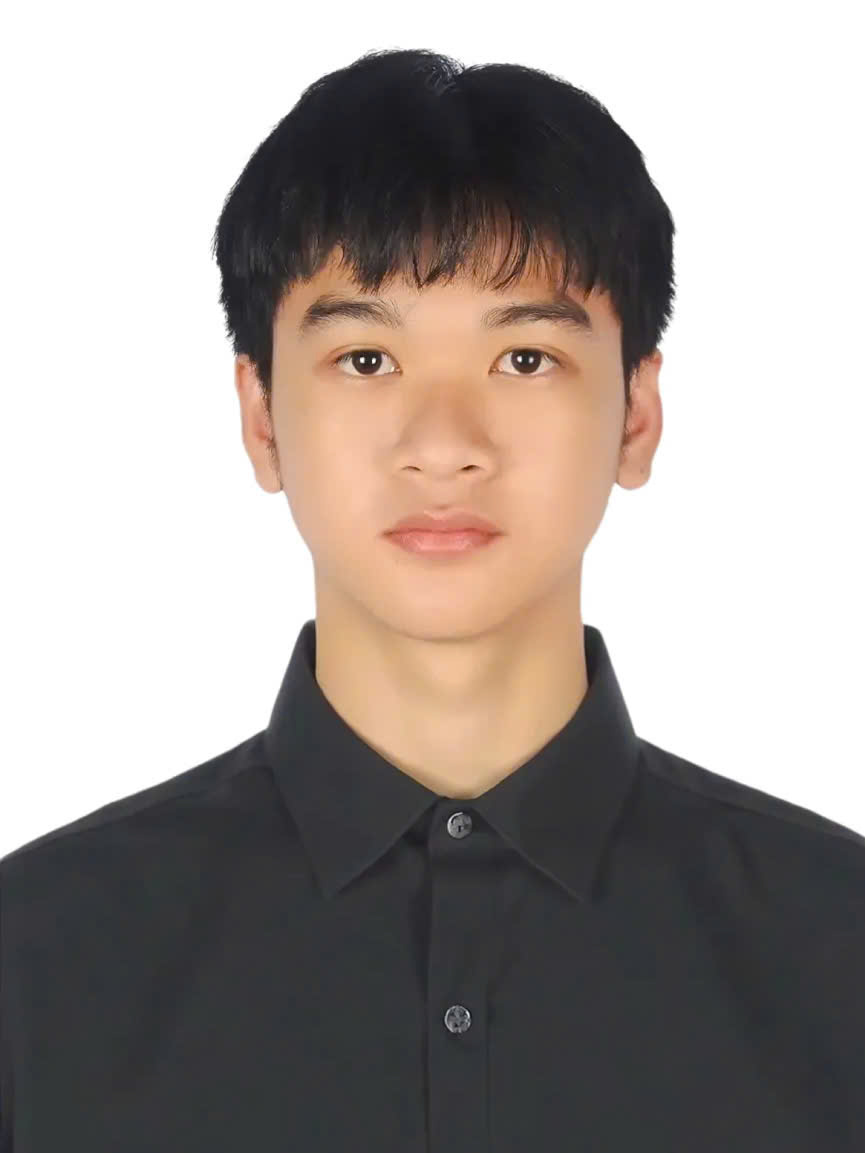
\includegraphics[width=2.4cm]{image/ProfileImage}
  \end{center}
\end{minipage}%
\begin{minipage}[c]{0.87\textwidth}
  \begin{center}
    {\Large \textbf{HA GIA PHUC}} \\[0.05cm]
    +(84) 846 2526 39 \ $|$ \ \href{mailto:Phucha2639@gmail.com}{\textcolor{black}{\underline{Phucha2639@gmail.com}}} \ $|$ \ \href{https://github.com/Giaphuc713}{\textcolor{black}{\underline{github.com/Giaphuc713}}} \\[0.05cm]
    DOB: 2004 \ $|$ \ Gender: Male

  \end{center}
\end{minipage}
\vspace{-0.5cm}



\section*{EDUCATION}
\vspace{-0.7em}
\hrule
\vspace{0.2em}
\begin{itemize}
    \item \textbf{University of Science, Vietnam National University Ho Chi Minh City (HCMUS)} \hfill 2022 -- 2026 
    \item \textbf{Major: Information Technology (Information Systems)} \hfill \textbf{GPA: 3.4 / 4}
\end{itemize}

\vspace{-0.4cm}

\section*{EXPERIENCE}
\vspace{-0.7em}
\hrule
\vspace{0.2em}

\noindent
\textbf{Daoukiwoom Innovation Company Limited} -- Fullstack Developer (Fintech domain) \hfill Aug 2025 -- July 2026
\begin{itemize}
    \item Participated in a cross-functional team of 8 members to develop a FinTech securities trading system, providing stable
    \item and user-friendly financial IT solutions for the Southeast Asian market.
    \item Operated under an Agile framework, managing tasks via Jira.
    \item Built and integrated backend services using \textbf{JavaScript}, \textbf{RESTful APIs}, focusing on API routing, service-to-service communication, authentication, authorization, and scalable backend design.
    \item Learned and applied SOLID principles to maintain a clean, decoupled, and maintainable architecture.
    \item Gained practical experience in containerization with Docker and automated CI/CD pipelines via Jenkins.
\end{itemize}

\vspace{-0.4cm}


\section*{GRADUATION PROJECT - AI AGENT STUDENT LEARNING ASSISTANT}
\vspace{-0.7em}
\hrule
\vspace{0.2em}
\textit{Tech Stack: LightRAG, MinerU, Knowledge Graph, Redis, GraphQL, Docker, Python } \hfill 01/2026 -- Present
\begin{itemize}
    \item Role: AI Developer – Team size: 4
    \item Implemented entity deduplication and sameAs entity linking to resolve duplicate entities across knowledge sources and improve Knowledge Graph consistency.
    \item Developed section-based document chunking to preserve document structure and contextual meaning, improving retrieval quality for LLM queries.
    \item Developed the web UI and integrated it with the LightRAG-based architecture to support AI Agent interactions and knowledge retrieval.
    \item Video Demo: \href{https://www.youtube.com/watch?v=nd5_PCkFh2w}{youtube.com}
\end{itemize}
\vspace{-0.4cm}

\section*{SKILLS}
\vspace{-0.7em}
\hrule
\vspace{0.2em}
\begin{itemize}
    \item \textbf{Programming Languages:} JavaScript/TypeScript, Python, C++, Java
    \item \textbf{Frontend:} React, Redux Toolkit, Tailwind CSS, HTML/CSS
    \item \textbf{Backend:} Node.js (Express), Java (Spring Boot)
    \item \textbf{Databases:} Microsoft SQL Server, MySQL, MongoDB, PostgreSQL
    \item \textbf{DevOps \& Tools:} Git, GitHub, Docker (basic), CI/CD (basic), RESTful APIs, Jenkins
\end{itemize}

\vspace{-0.4cm}


\section*{TECHNICAL PROJECTS}
\vspace{-0.7em}
\hrule
\vspace{0.2em}

\noindent
\textbf{Forum Platform} -- Personal Project\hfill 08/2026 -- 09/2026 \\
\textit{Tech Stack: Java, Spring Boot, Next.js, TypeScript, Tailwind CSS, PostgreSQL/Supabase, Claude, OAuth2}
\begin{itemize}
   \item A Reddit-inspired community forum platform with features for community management, post sharing, comments, and
content discovery.
   \item Built RESTful APIs using Java and Springboot for authentication, post creation, search, filtering, comments, and community membership.
   \item Developed a responsive and user-friendly forum interface using Next.js, TypeScript, and Tailwind CSS.
   \item Leveraged Claude to optimized application performance, API data fetching, and improve front-end quality
   \item Video Demo: \href{https://www.youtube.com/watch?v=iOXQ9wLZytc}{youtube.com} | Github: \href{https://github.com/Giaphuc713/Forum-Backend}{github.com/Forum-Backend}
\end{itemize}

\vspace{0.02cm}

\noindent
\textbf{Video Generation Platform} -- Team Project \hfill 03/2025 -- 07/2025 \\
\textit{Tech Stack: ASP.Net Core, React, Redux, Tailwind CSS, AI APIs, SQL Server, Entity Framework}
\begin{itemize}
   \item Combined audio and images into complete video outputs.
   \item Collected contents from Wikipedia, YouTube and leveraged third API services to generate images, audio.
   \item Develop React front-end for creating image, video, explore trending contents
   \item Video Demo: \href{https://www.youtube.com/watch?v=NpTDKAR5bkM}{youtube.com} | Github: \href{https://github.com/mquangcao/gen-vibe-video}{github.com}
\end{itemize}

\vspace{0.02cm}

\noindent
\textbf{Library Management System} -- Team Project \hfill 04/2024 -- 07/2024 \\
\textit{Tech Stack: SQL Server, Node.js, Javascript, Docker, Git, ReactJs, TailwindCss}
\begin{itemize}
    \item An online library system for managing book inventory, sales, and online ordering.
    \item Designed a user-friendly interface to enhance user experience.
    \item Created and modified stored procedures to handle inventory management, book sales, and monthly sales reporting.
    \item Implement JWT for authorization user and admin role.
    \item GitHub: \href{https://github.com/TranHuuTai1804/Book_MVC.git}{github.com/book-management}
\end{itemize}

\vspace{0.02cm}




\section*{CERTIFICATIONS}
\vspace{-0.7em}
\hrule
\vspace{0.2em}
\begin{itemize}
    \item \textbf{TOEIC Speaking \& Writingss:} 250 \hfill \textit{Jun 2025}
    \item \textbf{TOEIC Listening \& Reading:} 650 \hfill \textit{Dec 2024}
    \item \textbf{Udemy Certificate:} \href{https://www.udemy.com/certificate/UC-0f8f70ce-96fa-44e2-b836-cf4e8c49c22f/}{JavaScript From The Beginning 2.0} \hfill \textit{Aug 2025}
\end{itemize}

\vspace{-0.4cm}
\section*{ACTIVITY}
\vspace{-0.7em}
\hrule
\vspace{0.2em}
\begin{itemize}
    \item \textbf{IT Consultant Challenge 2024 – Netcompany} \hfill  \textit{Participant | 2024}
    \item \textbf{Spring Volunteer Campaign}\hfill\textit{Volunteer | 2025}

\end{itemize}

\end{document}

